\section[Environment]{Environments and code checks}
\sectionframe{03}{Environments and code checks}
  {Where does the agent run our code, and what checks it automatically?}
  {\faCubes}

% ------------------------------------------------------------------ conda
\begin{frame}[fragile,source={conda (2026), Managing environments · Anaconda (2025), Terms of service · Anthropic (2026), Claude Code docs}]{The classic setup: a conda environment}
  \begin{columns}[T,onlytextwidth]
    \begin{column}{0.42\textwidth}
\begin{codefile}[style=sh,basicstyle=\ttfamily\fontsize{7.2}{8.8}\selectfont]{environment.yml}
name: sem-seg
channels:
  - conda-forge
dependencies:
  - python=3.12
  - numpy
  - pandas
  - pytorch      # with CUDA builds
  - pytest
\end{codefile}
      % uv as a link to its repository, styled as the one over the screenshot on slide 24
      {\footnotesize Python-only projects:
       \href{https://github.com/astral-sh/uv}{\faGithub\enspace\underline{\fn{uv}}} is faster\par}
    \end{column}
    \begin{column}{0.55\textwidth}
\begin{terminal}[basicstyle=\ttfamily\fontsize{7.2}{8.8}\selectfont]{terminal}
$ conda env create -f environment.yml
$ conda activate sem-seg
$ conda run -n sem-seg pytest -q    # no activation
\end{terminal}
      \vskip1.4mm
      % an agent runs each command in a new shell, so an activation does not carry over
      \begin{tikzpicture}[x=1mm,y=1mm,
          sh/.style={anchor=west,inner sep=0pt,font=\ttfamily\fontsize{7}{8}\selectfont,text=termfg,
            execute at begin node={\setbox0\hbox{x}\spaceskip=\wd0\relax}},
          env/.style={anchor=west,rounded corners=0.8mm,inner xsep=1.1mm,inner ysep=0.7mm,
            font=\ttfamily\fontsize{7}{8}\selectfont\bfseries,text=white}]
        \node[anchor=north west,inner sep=0pt,font=\footnotesize\bfseries,text=udsdark] at (0,0)
          {an agent session: a new shell for every command};
        \foreach \i/\c/\e/\col in {1/{conda activate sem-seg}/{sem-seg}/udsblue,
            2/{pytest -q}/{not sem-seg}/udsred,3/{conda run -n sem-seg pytest -q}/{sem-seg}/udsblue} {
          \pgfmathsetmacro\y{-1.8-\i*6.2}
          \fill[termbg,rounded corners=1mm] (0,\y+2.4) rectangle (57,\y-2.4);
          \foreach \d [count=\j] in {termdot1,termdot2,termdot3} \fill[\d] (\j*1.7,\y) circle (0.45);
          \node[sh] at (6.8,\y) {\textcolor{termgreen}{\$} \c};
          \node[env,fill=\col] at (59,\y) {\e};
        }
      \end{tikzpicture}\par\vskip1.4mm
      {\footnotesize or: activate first, then start the agent\par}
    \end{column}
  \end{columns}
  \note{\textbf{12:50--13:50}\par
    Most of us use conda.\par
    An environment.yml lists channel and packages; conda builds the environment, activate enters it.\par
    Three things matter once an agent works in it.\par
    Each command an agent runs starts a fresh shell, so an activation does not carry over;
      Claude Code's documentation says to activate the environment before launching it, and
      conda run executes a command in an environment without activating it.\par
    An environment.yml without versions drifts: rebuilt next year, it resolves to different
      packages; conda 26.5 and later export a lockfile with exact versions, conda-lock does the
      same for older versions.\par
    And the channel: PyTorch's conda packages now come from conda-forge, Miniforge's only channel.\par
    Anaconda's own channel has terms of service, free for academic use under conditions, that
      count AI agents and automated jobs as users; check with the university's IT before relying
      on it.\par
    For Python-only projects uv is faster; A4 and A5 in the appendix show it.}
\end{frame}

% ------------------------------------------------------------ three tools
\begin{frame}[source={Astral (2026), Ruff documentation · mypy documentation · Microsoft (2026), Pylance README}]{Ruff, mypy and Pylance}
  \begin{tikzpicture}[x=1mm,y=1mm,
      col/.style={anchor=base,inner sep=0pt,font=\footnotesize\bfseries,text=udsdark,align=center,
        text width=24mm},
      tool/.style={anchor=base west,inner sep=0pt,font=\small\bfseries,text=udsdark},
      what/.style={anchor=base west,inner sep=0pt,font=\scriptsize,text=udsgrey},
      yes/.style={circle,fill=udsblue,minimum size=3.8mm,inner sep=0pt},
      no/.style={circle,draw=udsgreylight,line width=0.6pt,minimum size=2mm,inner sep=0pt}]
    \useasboundingbox (0,0) rectangle (144,-49.4);
    % where it runs; with a text width a node's base is its first baseline, so the heads share both
    \foreach \x/\h/\s in {58/VS Code/in the editor,83/terminal/you and the agent,
        108/pre-commit/before each commit,133/CI/on every push}
      \node[col] at (\x,-2.1) {\h\\[-0.4mm]{\scriptsize\mdseries\color{udsgrey}\s}};
    \draw[udsgreylight,line width=0.5pt] (0,-7.6) -- (144,-7.6);
    % one row per tool: what it does, and a dot where it runs, centred on the row
    \foreach \i/\t/\w/\a/\b/\c/\d in {
        0/Ruff/{lint and format}/yes/yes/yes/yes,
        1/mypy/{type check}/yes/yes/no/yes,
        2/Pylance/{VS Code's language server}/yes/no/no/no} {
      \pgfmathsetmacro\y{-13.6-\i*12}
      \node[tool] at (0,\y+0.95) {\t};
      \node[what] at (0,\y-2.65) {\w};
      \node[\a] at (58,\y) {};
      \node[\b] at (83,\y) {};
      \node[\c] at (108,\y) {};
      \node[\d] at (133,\y) {};
      \draw[udsgreypale,line width=0.5pt] (0,\y-6) -- (144,\y-6);
    }
    \node[anchor=base west,inner sep=0pt,font=\footnotesize,text=udsdark] at (0,-48.6)
      {type hints such as \fn{n\_folds: int}: read by mypy and Pylance, ignored when the code runs};
  \end{tikzpicture}
  \note{\textbf{13:50--14:40}\par
    Three tools that read the code without running it.\par
    Ruff, from the makers of uv, is a linter, which flags likely mistakes such as an unused
      import, and a formatter; it replaces Flake8, Black and isort.\par
    It can run before every commit, through pre-commit, and in CI, continuous integration:
      checks that a server such as GitHub runs on every push.\par
    mypy checks types against the hints in the code, the reference for the command line and
      CI.\par
    Pylance, built on Pyright, powers VS Code's completion and navigation and checks types as
      you type once type checking is switched on; its default is off.\par
    It also flags packages missing from the selected environment, a common cause of red
      underlines.\par
    Pylance runs only in Microsoft's VS Code.}
\end{frame}

% ---------------------------------------------------------- in VS Code
\begin{frame}{What it looks like in VS Code}
  \begin{columns}[T,onlytextwidth]
    \begin{column}{0.7\textwidth}
      \begin{tikzpicture}
        \node[anchor=south west,inner sep=0pt,draw=udsgreylight,line width=0.4pt] (img) at (0,0)
          {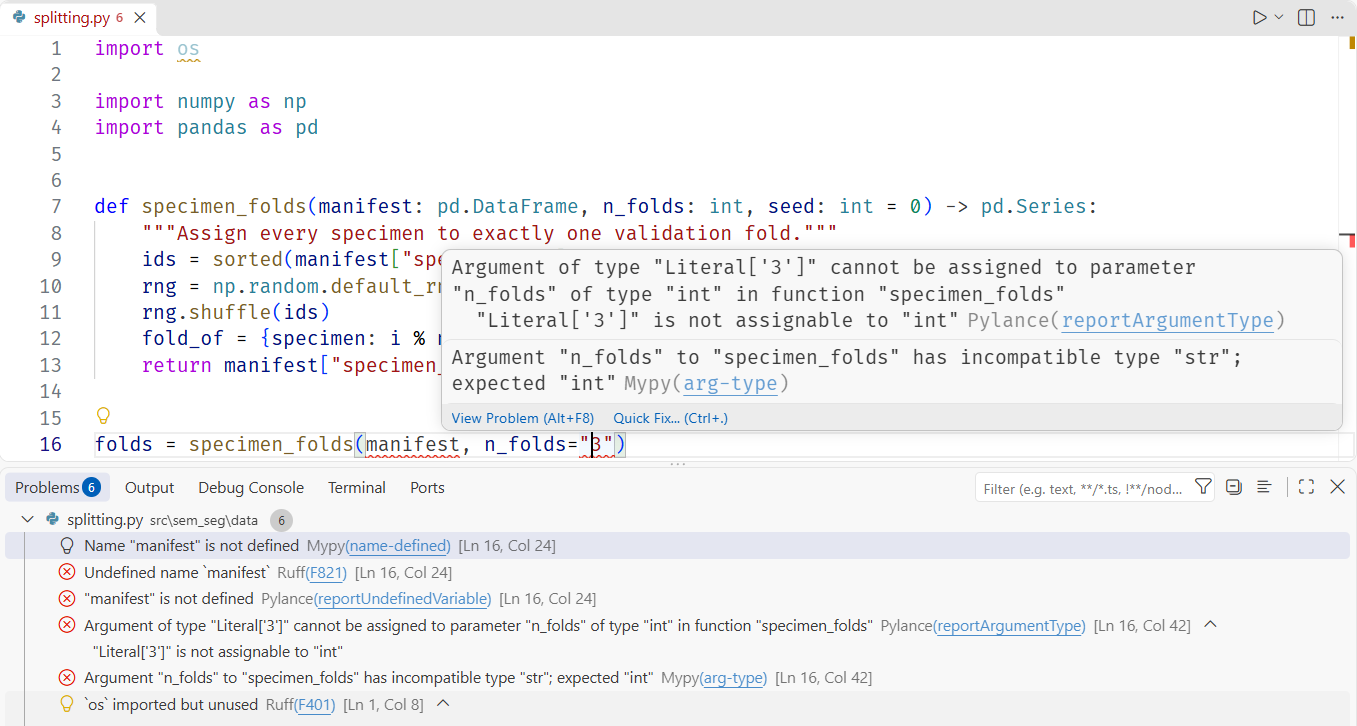
\includegraphics[width=\linewidth]{assets/screens/vscode-lint.png}};
        \begin{scope}[x={(img.south east)},y={(img.north west)},
            mk/.style={circle,fill=udsred,text=white,font=\scriptsize\bfseries,inner sep=0pt,minimum size=4mm}]
          \node[mk] at (0.179,0.963) {1};
          \node[mk] at (0.849,0.698) {2};
          \node[mk] at (0.111,0.328) {3};
        \end{scope}
      \end{tikzpicture}
    \end{column}
    \begin{column}{0.27\textwidth}
      \footnotesize
      \begin{enumerate}\setlength\itemsep{2mm}
        \item Ruff: unused import (\fn{F401}), undefined name (\fn{F821})
        \item Pylance and mypy: a string passed as \fn{n\_folds}
        \item Problems panel: every finding, with its tool and rule
      \end{enumerate}
    \end{column}
  \end{columns}
  \note{\textbf{14:40--15:30}\par
    A real screenshot: VS Code 1.142 with the Ruff, Pylance and Mypy extensions on a
      deliberately broken version of our split function.\par
    Squiggles mark the unused import, the undefined name and the wrong argument type; hovering
      shows the message and which tool raised it.\par
    The Problems panel lists all six findings, each with its tool and rule, so you can look up
      or switch off a rule.\par
    The agent sees the same findings when it runs the tools from the terminal.}
\end{frame}

% ------------------------------------------------------------ set up once
\begin{frame}[fragile,source={Astral (2026), Ruff: editor setup · Microsoft (2026), Mypy Type Checker; Pylance README}]{Set them up once}
  % left: the tools on the command line; right: the same tools in VS Code
  \begin{columns}[T,onlytextwidth]
    \begin{column}{0.475\textwidth}
\begin{codefile}[style=sh,basicstyle=\ttfamily\fontsize{7}{8.4}\selectfont]{pyproject.toml}
[tool.ruff]
line-length = 100       # rules: Ruff's defaults

[tool.mypy]
python_version = "3.12"
\end{codefile}
      \scriptsize\renewcommand\arraystretch{1.4}\setlength\tabcolsep{3pt}
      \begin{tabularx}{\linewidth}{@{}>{\bfseries}l>{\ttfamily}X@{}}
        \toprule
        Install        & conda install -c conda-forge ruff mypy\\
        \midrule
        Lint and fix   & ruff check --fix\\
        Format         & ruff format\\
        Types          & mypy src\\
        \bottomrule
      \end{tabularx}
    \end{column}
    \begin{column}{0.495\textwidth}
\begin{codefile}[basicstyle=\ttfamily\fontsize{7}{8.4}\selectfont]{.vscode/settings.json}
"[python]": {
  "editor.defaultFormatter": "charliermarsh.ruff",
  "editor.formatOnSave": true,
  "editor.codeActionsOnSave": {
    "source.fixAll": "explicit",
    "source.organizeImports": "explicit"}},
"python.analysis.typeCheckingMode": "standard",
"mypy-type-checker.importStrategy":
  "fromEnvironment"
\end{codefile}
      \footnotesize
      \begin{itemize}\setlength\itemsep{1mm}
        \item VS Code extensions: Python (brings Pylance), Ruff, Mypy Type Checker
        \item pick the environment: \emph{Python: Select Interpreter}
        \item the same commands go into \fn{AGENTS.md} and CI
      \end{itemize}
    \end{column}
  \end{columns}
  \note{\textbf{15:30--16:30}\par
    Set up once per repository, then it runs by itself.\par
    The tool settings live in pyproject.toml, which works for conda projects too.\par
    One conda command installs both; by hand, three commands lint, format and type-check.\par
    In VS Code, install the Python extension, which brings Pylance, plus the Ruff and Mypy Type
      Checker extensions, and select the project's environment.\par
    The workspace settings make Ruff format and fix on every save, switch Pylance's type
      checking on, and make the Mypy extension use the mypy installed in the environment rather
      than the older copy it bundles.\par
    The same commands go into AGENTS.md, so the agent runs them too, and into CI.}
\end{frame}
